\documentclass[11pt]{article}
\usepackage{icmlko}
\begin{document}

\title{전이의 값이 매겨졌다 --- 판 0.0117 을 내면 음수가 0 이 된다}
\author{월드모델 실험실}
\date{노트 399 · 2026년 8월 2일}
\maketitle

\begin{abstract}
노트 398이 옆방 도메인(KR 만화)에서 전이가 $-0.1261$ 인 것을 보이고, 남은
설명 하나를 지목했다 --- \textbf{도메인 원핫}. F18 은 도메인마다 원핫을
하나씩 갖고 모르는 도메인에는 전부 0 을 준다. 사전 등록했다: \emph{원핫이
범인이면 그것을 빼면 KR 이 오르고 JP 가 내려간다.}

\begin{center}
\begin{tabular}{lrr}
\hline
 & KR 만화(안 본 도메인) & JP 만화(학습에 듦) \\
\hline
원핫 있음 (챔피언) & $-0.1261$ & $+0.3196$ \\
\textbf{원핫 없음} & $\mathbf{+0.0797}$ & $+0.3202$ \\
\hline
\end{tabular}
\end{center}

\textbf{절반 맞고 절반 틀렸다.} KR 은 예측대로 올라 \textbf{0 을 넘는다}.
그런데 JP 는 안 내려간다($+0.3196 \to +0.3202$). \textbf{원핫은 학습에 든
도메인에 이득을 주는 게 아니라 안 본 도메인에 해를 준다.}

\textbf{그러면 값이 얼마인가.} 짝 12뽑기로 쟀다: 판
$\mathbf{-0.0117}$ · SD 0.0034 · \textbf{0/12}. 판이 결정적으로 뺀다고
한다.

\begin{center}
\textbf{판 $0.0117$ 을 내면 전이가 $-0.1261 \to +0.0797$, 즉
$+0.2058$ 만큼 산다.}
\end{center}

\textbf{맞바꿈이 처음으로 수로 나왔다.} 그리고 이것은 이 실험실의 규약이
혼자 못 정하는 종류다 --- \textbf{판은 ``빼라''고 하고 목표는 ``빼자''고
한다.} 판은 학습에 든 도메인 안의 수이고(노트 398), IP 파운데이션이라는
목표는 그 밖을 주장한다.

\textbf{챔피언은 안 바꾼다.} 순위 규칙이 판이고, 전이 증거가 아직 도메인
둘(앱 · KR 만화)뿐이다. \textbf{대신 값을 대장에 박아 둔다} --- 다음에
전이 점이 서넛 더 쌓이면 이 수가 결정을 정한다.
\end{abstract}

\section{원핫이 무엇을 하나}

\texttt{F18.fit} 은 도메인마다 열을 하나씩 만들어 그 도메인 행에 1 을
준다. 학습에서는 도메인별 절편 노릇을 해 ``이 도메인은 라벨이 대체로
높다/낮다''를 담는다. 예측에서는 아는 도메인이면 그 열을 켜고,
\textbf{모르는 도메인이면 전부 0 을 준다.}

전부 0 은 학습에 한 번도 안 나온 좌표다. 나무가 그 좌표에서 무엇을 하는지
아무도 정하지 않았고, 그래서 KR 만화에서 \emph{거꾸로} 줄을 세웠다는 것이
노트 398의 관측이다.

\begin{figure}[t]
\centering
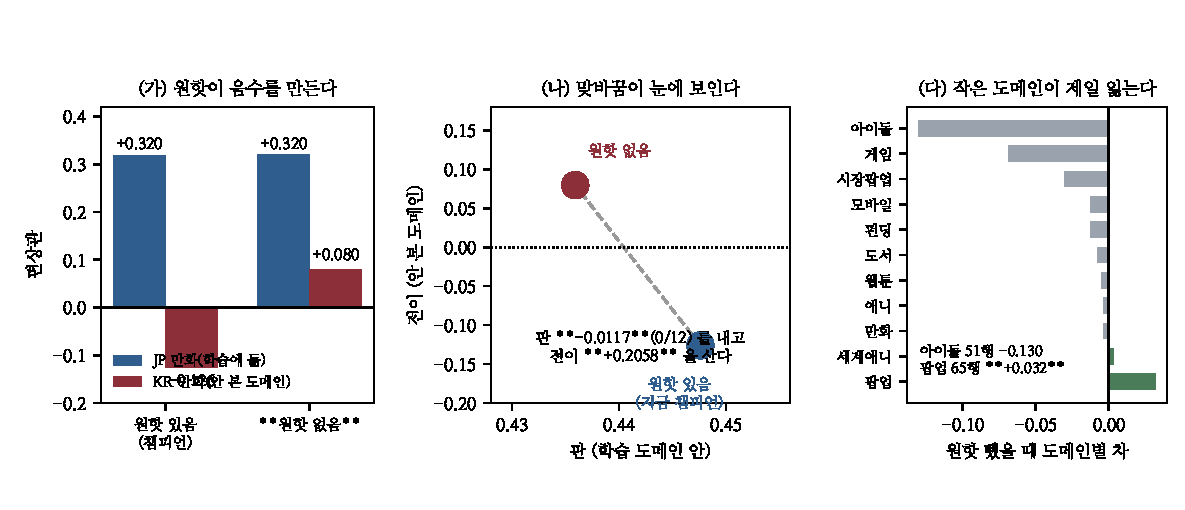
\includegraphics[width=\linewidth]{figs/fig399.pdf}
\caption{\textbf{(가)} 원핫을 빼면 KR 이 $-0.13 \to +0.08$ 로 오르고 JP 는
안 움직인다. \textbf{(나)} 맞바꿈 --- 판 $0.0117$ 을 내고 전이 $0.2058$ 을
산다. \textbf{(다)} 원핫을 뺐을 때 도메인별 손익. 유보가 작은 도메인이 제일
잃는다.}
\label{fig:main}
\end{figure}

\section{쟀다}

원핫 열만 안 만드는 \texttt{NoOneHot} 을 F18 에서 상속해 만들었다 --- 나머지
(부스팅 · 배깅 $K{=}32$ · 순위 평균)는 한 글자도 안 바꿨다. 씨앗 여섯 평균,
공유 축 다섯, 날짜 통제 편상관(노트 397 · 398과 같은 절차).

\textbf{전이 쪽.} KR $-0.1261 \to +0.0797$. \textbf{$0$ 을 넘는다} ---
음수 전이가 사라진다. 다만 $\pm0.056$ 이라 양수라고 단언은 못 하고,
노트 397의 앱($+0.0824$)과 같은 자리다.

\textbf{학습 도메인 쪽.} JP 만화 $+0.3196 \to +0.3202$ --- 안 움직인다.
\textbf{사전 등록의 절반이 틀렸다.} 원핫이 만화에 주던 이득은 사실상
없었다.

\textbf{판 쪽.} 짝 12뽑기 $-0.0117$ · 0/12. 어디서 잃나 보면
\textbf{유보가 작은 도메인}이다 --- 아이돌 $-0.1301$(51행) · 게임
$-0.0685$(180행) · 시장팝업 $-0.0300$(126행). 원핫은 표본이 적은 도메인의
절편을 대신 잡아 주고 있었다. \textbf{반대로 팝업은 $+0.0319$(11/12)로
오른다} --- 65행인데 오르는 것이 뜻밖이고 관측으로 둔다.

\section{규약이 혼자 못 정한다}

이 실험실의 순위 규칙은 유보 표본의 판 $\rho$ 다. 그 규칙대로면 이 변경은
$0/12$ 로 기각이다. \textbf{그런데 노트 398이 판의 뜻을 좁혔다} --- 판은
\emph{학습에 든 도메인 안에서의} 평균이다. IP 파운데이션이라는 목표는 그
밖을 주장하고, 그 밖에서 지금 챔피언은 $-0.13$ 이다.

\textbf{두 수가 반대를 가리킨다.} 판은 원핫을 지키라 하고 목표는 빼라 한다.
이것은 관문이 푸는 문제가 아니라 \emph{무엇을 재느냐}의 문제다.

\textbf{그래서 안 바꾼다 --- 지금은.} 이유가 둘이다. \textbf{첫째, 전이
증거가 도메인 둘뿐이다}(앱 $+0.08$ · KR 만화 $-0.13$). 둘로 순위 규칙을
갈아엎을 수 없다. \textbf{둘째, 원핫 없는 쪽도 전이가 $+0.08 \pm 0.056$
이라 0 과 못 가른다} --- 음수를 없앤 것이지 전이를 만든 것이 아니다.
``해를 없앴다''와 ``이득을 얻었다''는 다르다.

\textbf{대신 값을 박아 둔다.} 전이 점이 서넛 더 쌓이고 그중에 원핫 없는
쪽이 뚜렷이 양수인 사례가 나오면, 이 $0.0117$ 이 치를 값이다.

\section{남은 것}

\begin{center}
\begin{tabular}{lll}
\hline
항목 & 왜 값이 큰가 & 어떻게 \\
\hline
CN 만화 352행 & 세 번째 짝이 같은 자리에 있다 & 노트 398 절차 그대로 \\
원핫을 반만 & 맞바꿈 곡선의 가운데 점 & 원핫에 축소를 걸어 본다 \\
작은 도메인이 왜 잃나 & 절편을 대신 잡아 주고 있었다 & 도메인 평균만 따로 주고 재본다 \\
판의 이름 & 노트 398이 남긴 것 & 대장 표기를 ``판(학습 도메인 안)'' 으로 \\
\hline
\end{tabular}
\end{center}

\end{document}
